\documentclass[parskip=full]{scrreprt}
% Paket um vordefinierte Texte (z.B. "Inhaltsverzeichnis") auf Deutsch zu übersetzen
\usepackage[english]{babel}

% Paket um Schriftarten festzulegen (für XeLaTeX)
\usepackage{fontspec}

% serifenfreie Schriftart Arial festlegen
% \setsansfont{}ð

% serifenfreie Schriftvariante verwenden
\renewcommand{\familydefault}{\sfdefault}

% Paket um Grafiken (JPG, PNG, PDF) einzubinden
\usepackage{graphicx}

% Paket für Zeilenabstand
\usepackage{setspace}

% Paket für korrekte Anführungszeichen
\usepackage{csquotes}

% Paket für selbst definierte Kopf- und Fusszeilen
\usepackage{scrlayer-scrpage}

% Pakte für Zitate und Bibliografie
\usepackage{biblatex}

\addbibresource{literature.bib}

% Paket zum Erzeugen von Platzhaltertext
\usepackage{lipsum}

% Code below courtesy of chatgpt-4o on 2024-06-25

% Package for changing theorem style
\usepackage{amsthm}

% Code to change theorem styling
\setlength{\topsep}{0.1em}
\setlength{\partopsep}{0.1em} % Extra space above theorem if at the beginning of a list
\setlength{\parsep}{0.1em} % Space between paragraphs within the theorem

% End of code courtesy of chatgpt-4o

% Packge for code highlighting
\usepackage{listings}


\usepackage{courier}        % For monospace font
\usepackage{xcolor}         % For background color

\lstdefinestyle{customverilog}{
    language=verilog,                    % Set language to Verilog/SystemVerilog
    basicstyle=\ttfamily\scriptsize,                % Monospace font
    breaklines=true,                     % Break long lines if necessary
    numbers=left,                        % Line numbers on the left
    numberstyle=\tiny,                   % Line numbers in tiny font
    backgroundcolor=\color{gray!10},     % Light gray background
}


\lstset{style=customverilog}


% Package for hyperlinks
\usepackage[hidelinks]{hyperref}

% Package for float placement
\usepackage{float}

% noitemsep
\usepackage{enumitem}
\setlist{nolistsep}
\setlist{noitemsep}

% tikz
\usepackage{tikz}
\usepackage{tikz-timing}
\usetikzlibrary{shapes.geometric, arrows.meta}
\usepackage{caption}
\DeclareCaptionType {timingdiag}[Timing diagram][List of Timing Diagrams]

\renewcommand*{\ttdefault}{cmtt}

% listings

% Schmale Seitenränder festlegen
\KOMAoption{DIV}{15}

% Text auf Titelseite festlegen
\subject{Maturapaper}
\title{Designing and implementing an 8-bit Computer Architecture in Verilog}
\author{Rufus Spyra\vspace{1cm}\\
Supervised by \\
Stefan Rothe}

\publishers{
\includegraphics{logo}\vspace{1cm}\\
Gymnasium Kirchenfeld\\
Divison MN}

% selbst definierte Kopf- und Fusszeile
\lohead{Maturapaper}
\rohead{\input{jobid}, \input{gitbranch.tex}@\input{githash}}
%\rohead{\theauthor}
\cofoot{\thepage}

% Zeilenabstand festlegen
\singlespacing
%\onehalfspacing
%\doublespacing

% Trennlinie für Kopfzeile
\KOMAoption{headsepline}{off} % oder on

% Trennlinie für Fusszeile
\KOMAoption{footsepline}{on} % oder on

\begin{document}

\maketitle

\tableofcontents

\chapter{Introduction}
My fascination of retro computers sparked when I watched an online show about building an 8-bit computer on a breadboard. After countless hours of explanations, the viewer was rewarded with a blinking monster of wires and chips, functioning together to reach a goal. Ever since I watched this show \cite{beneater}, I wanted to design and build a computer like this. Over a couple of years I got further invested in the topic, fascinated by the initial impact of the first introduction of 8-bit computers in the 1970s and the sheer complexity of computer chips, I wanted to design my own computer architecture and simulation - just like if it was a real chip design, that is supposed to be physically manufactured on silicon. Unfortunately, physical construction, be it in silicon, or any other medium, was quickly ruled out due to overwhelming time efforts and costs. Manufacturing a chip in silicon not only requires physical manufacturing capabilities but also highly specialized software, that is proprietary and not intended for amateur usage. 

The goal of this project is to design a computer architecture following the process and constraints of a chip design up until silicon or hardware design and manufacturing.

Following my inspiration, the architecture that is to be designed shall be kept very simple. This is achieved by limiting the bus width to 8-bits. Furthermore, the architecture shall follow the classic von Neumann Architecture and be Turing equivalent.  


\section{Chip Design} \label{sec:chip-design}
To move from idea to a finished product, chip designs follow a specific flow. Although different sources may describe this process differently. It is clear however, that this process is intended to be highly sequential and linearized.

At first, all top level requirements must be clearly established, which are then further broken down in smaller and smaller requirements. This step is referred to as "System specification and architectural design".

At some point these requirements then reach the point where, they specify functional details of the chip/architecture, such as compartmentalization and signalling. This is then referred to as "Functional design." With enough specificity these requirements can then be transferred into computer aided designs utilizing hardware description computer languages, a process called "Logic design". This logic design can then be transferred, either manually or by sophisticated computer programs, into logic gates and a silicon layout, during the "physical design"  process. Before this is step is started, the logic design is tested against the defined requirements to ensure that it implements them correctly, which is called "Verification and Validation". Any mistakes in the logic design would translate into faulty silicon, making these mistakes extremely costly \cite{chipdesignflow1} \cite{chipdesignflow2}. The generated design would then be handed off to production.

As previously stated, this project shall treat all steps up until and with "Verification and Validation". The collection of this process is sometimes also referred to \textit{front end design}.

\subsection{Requirements}
\textit{Requirements engineering} describes the process of not only establishing high level requirements, e.g. the project goals, but also the translation into more specific and precise low level requirements. The formulation of useful requirements is essential to the success of a project. The value of a requirement lies in its ability to translate what the author wanted into what an engineer made of it. This means requirements must be unambiguous, correct and ideally precise and concise \cite{requirementsengineering}.

\subsection{Hardware Description Languages}
With the development of highly complex chip designs in the late 20th century, further and further abstraction of the logic design process was required, ensuring that all stakeholders knew the exact specifications of the design at any point. Whilst the earliest chip designs were drawn by hand and later transferred onto silicon by photolithography, chip designs nowadays are first written in an abstract computer language; a Hardware Description Language. This hardware description can then be transferred into silicon either manually or automatically.  Apart from also allowing separation, modularity and reusability of components, this description later also allowed for simulation of the design. This simulation brought the key advantage of being able to be tested against requirements to check for errors \cite{histverilog} \cite{1214355}.

\subsection{Automated Testing}
Nowadays, this automated testing process is handled by software frameworks designed for this purpose. These software frameworks instantiate and execute the simulation of the \textit{design under test} on top of \textit{testbench} code. The testbench models behaviour of external components which is applied onto the design under test. The response of it is then compared to expected results and validated to ensure the design meets all requirements.

While requirements should cover all of an architectures' logic design implementation, some pieces of code could be not covered by tests. To ensure that all code is tested, testing frameworks provide \textit{code coverage analysis tools}. The tools count activations of specific lines of code. This activation count can then be used to produce a visual report that shows all used lines of code, highlighting areas that aren't covered by test.

Automated testbenches can be generally be split into two categories: exhaustive testing and directed testing. Exhaustive testbenches test by supplying every possible test input to the design under test. Most of the time this is not required, as if it works for one input it should work for any other input. Exhaustive testing does also require significantly more time. Consequently, testbenches shall be written in a directed fashion. 

\cite{verilogtestbench} \cite{exhaustivetesting} \cite{directedtesting}


\subsection{Development Operations and Version Control Systems}
To track development over time \textit{version control systems} are used in basically every software project. Closely tied to most version control systems are \textit{development operations}. The goal of development operations is to connect the software development closer to its operations. In many projects these operations are e.g. the continuous deployment of code changes and the execution of automated tests. Applied to this project, the development operations signify the execution of automatic testing of code changes as soon as changes are registered with the version control system. 

This combination allows for tracking and tracing the development process over time and provides quick feedback to engineers on problems arising in the code.

\section{Computer Architecture Design}

\subsection{Turing equivalence}
One of the most important concepts in computer science was established in 1936 by British mathematician Alan Turing. He described an algorithm that is \texttt{computationally universal}. To be computationally universal, an algorithm needs to be able to execute any other algorithm \cite{britannicaturing}.

Given a number of theoretical problems in computer science an algorithm like this cannot exist. The most prominent example for this is the Halting Problem. It describes, that given computational universality, an algorithm needs to exist, that can determine another algorithms runtime \cite{haltingproblem}, which, e.g. for an algorithm that could run infinitely, is not possible.

Computer science introduced the term \textit{Turing equivalent} to describe a machine that is exactly as powerful as the machine Turing described in his 1936 paper. If a computer architecture is Turing equivalent to a Turing machine, it can perform any algorithm that a modern computer can as well, given enough, theoretically infinite, memory, power and time.

Generally speaking, to be Turing equivalent to a Turing machine, an architecture or machine must have the following capabilities \cite{beneaterturing}:
\begin{itemize}
  \item Have the ability to modify memory
  \item Have the ability to execute conditionally based on memory
  \item Have infinite time and memory
\end{itemize}


\subsection{The von Neumann Architecture} \label{subsec:vna}
In 1945 John von Neumann, an American mathematician, developed a concept for a computing device. What made this concept prevail into modern computing was its general purpose design. The executing program is intended to be exchangeable to fit the problem that is to be solved.

The truly pioneering approach of the von Neumann Architecture was to store the instructions in the same physical memory as the operands, thus accessed in the same way, as the data which simplified the programming process by allowing other programs (compilers, interpreters) to translate from more abstract languages. As instructions and data are stored in the same memory, they must also share the same physical bus. This however leads  to a phenomenon known as the \textit{von Neumann bottleneck}, where the bus and memory are the limiting factor in the speed of the computer. It arises because both the instruction fetch, and all data operations must share the same bus and can only occur one after the other, creating a point of congestion. 

The architecture is split up into four modules, that each serve a distinct purpose. The \textit{arithmetic logic unit} (ALU) handles all mathematical operations on data. All data is stored in the \textit{memory}. Interaction with users and/or other systems occur through the \textit{input/output unit}. All modules are orchestrated by the \textit{control unit} (CU) which controls the modules through the \textit{control bus}. The modules then exchange data through the \textit{data and address bus} \cite{vonneumann1} \cite{vonneumann2}.

\begin{figure}[H]
  \begin{center}
    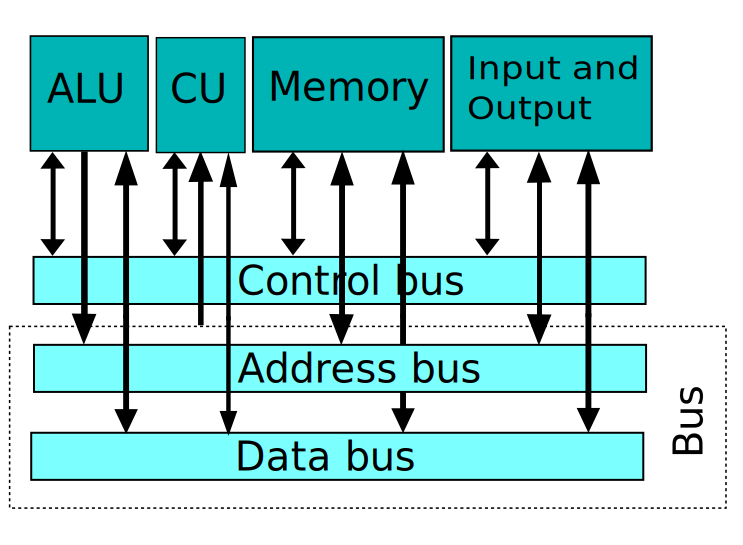
\includegraphics[width=0.5\textwidth]{figures/VNA}
  \end{center}
  \caption{The Von Neumann Architecture. Adapted from \cite{fig-vna}}\label{fig:vna}
\end{figure}

For this project, the data bus shall be referred to instead as the \textit{operand bus}, as its primary purpose is carrying operands. The combined address and operand bus shall be referred to as \textit{data bus}.

\subsection{Instruction Hierarchy}
The control unit controls the computer based on a \textit{program}. Each program serves a distinct purpose, e.g. calculating a series of numbers. It consists of multiple \textit{macro instructions}, which in return consist of multiple \textit{micro instructions}. Macro instructions perform, aligned with the von Neumann Architecture, an operation on a single \textit{data word}, such as overwriting it, or storing it somewhere else. A Micro instructions refers to the state of all control signals, e.g. if a component is reading or writing to the bus. Although it is possible to program a computer solely with micro instructions, it would be extremely inefficient, as the program code would be strongly repetitive \cite{malvino1983a}.

A collection of macro instructions is referred to as an \textit{instruction set}. 

\section{Tools} \label{sec:tools}

The most popular flavour of such a \textit{hardware description language} is Verilog, as defined in \textit{IEEE Std 1800-2023} \cite{10458102} and its extensions. Given widespread professional use of Verilog, more specifically the Verilog superset SystemVerilog, seemed to be the best option for this project as a large amount of information and guides on the topic exist. The terms SystemVerilog and Verilog will be used interchangeably. 

As the IEEE Standard only defines the language's syntax, a Verilog tool suite is required. Although previous experience in the usage of Verilog exists, expertise on the intricacies of Verilog simulation is still limited. It was thus decided based on the integration with other tooling, as to which suite is to be used. 

The key feature of the chosen suite, which is called \textit{Verilator}, is the compilation of the Verilog code to a binary and the generation of an interface to C++. Having an interface to C++ enables much more complex behaviours to be modelled in a simpler manner, such as reading test data from a file. Additionally, apart from being able to rely on previous experience in C++, it also allows me to make use of a vast ecosystem of testing, code coverage and development operations frameworks. Furthermore, the suite is available under the LGPL licence, allowing me to use it free of charge. I chose the GoogleTest framework for automated testing procedures. Most testing frameworks in essence do the same thing, although there are small nuances that differ from one to the other. 

Verilator also provides interfaces to coverage analysis tools by generating \textit{dumpfiles}. Dumpfiles contain the data of all signal values in the simulation across time and can be read by "digital oscilloscopes" like GTKWave. These can then be used to debug and understand the simulation, in case errors exist \cite{verilatoroverview}.

Git and GitLab are used as the version control system and development operations platform.

\subsection{Verilog Crash Course}
This section is not intended to be an exhaustive guide to Verilog, but only highlights the most important features and concepts relevant for this project. It is based on an internet guide \cite{verilogcourse}.

What differentiates simulated Verilog from other computer languages is its non-linear execution and its lack of a main function. Verilog files are not necessarily executed from top to bottom, but execution is based on propagation of signals throughout the interconnected modules. 

A module is declared with the \texttt{module} keyword. To complete a declaration the module must be named and ports specified. Ports are the connections going in and out of a module. They can either be an \texttt{input}, an \texttt{output} or bidirectional, denoted by \texttt{inout}. Ports are then specified like any other variable, by specifying the data type, length and name. For this paper usage of data types shall be limited to, \texttt{wire}, \texttt{reg}, \texttt{bit}, \texttt{logic} and for readability reasons \texttt{enum}. After the declaration of the ports the body of the module is defined, which contains the module logic.

\begin{lstlisting}[language=Verilog, caption=Module definition]
module <module_name> (
  input wire <input_name>,
  output reg <output_name>
);
<module_body>
endmodule
\end{lstlisting}


Most digital circuits are based around a clock signal and thus have to execute operations at every clock cycle. Verilog provides a way to model this with \texttt{always} blocks. Once the condition in the bracket is met, the code block is executed. Apart from simple boolean conditions, the block can also be executed at the rising and falling edge of a signal by using the \texttt{posedge} and \texttt{negedge} keywords.

\begin{lstlisting}[language=Verilog, caption=Always block definition]
always @(<condition>) begin
  <always_body>
end

\end{lstlisting}

As for the logic, the Verilog standard specifies if-blocks, loops, case statements and various logic and arithmetic operators comparable to other computer or programming languages. Unlike other languages, there are multiple types of assignments in Verilog. The easiest to understand is the continuous assignment with the \texttt{assign} keyword. This continuously assigns the value of the right-hand side to the left-hand side comparable to physical wires being connected together through logic gates. If the input changes, the output will change with it nearly instantaneously. The blocking assignment, denoted by the \texttt{=} operator, is used to assign values to variables instantaneously, like in other programming languages. The non-blocking assignment, denoted by the \texttt{<=} operator, only actually assigns the value to the left-hand side once the timing step, so every calculation in the current time step, is finished. 


The SystemVerilog standard also specifies a number of additional functions that are not synthesizable, so cannot be translated into hardware, but are useful for simulation, such as \texttt{\$display} and \texttt{\$finish}. As they are not synthesizable, they shall not be used, for this project. These features can be handled by the \texttt{C++} testbenches.



\subsection{Development Environment}
To reproduce the development environment for this project, the following packages need to be available in \texttt{PATH}. I suggest to use Debian 12. 

\begin{itemize}
  \item verilator@5.24
  \item a C++ tool chain (e.g. GCC)
  \item CMake
  \item a CMake generator (e.g. ninja)
\end{itemize}  

\begin{lstlisting}[caption=Build instruction, language=bash, label=lst:build]
# Make a new folder in the source directory
mkdir build
cd build
# Initalize CMake with the chosen generator. Here: ninja
cmake .. -GNinja
# Execute it
ninja

# To perfrom the tests execute ctest.
ctest

# To generate coverage info execute verilator_coverage
verilator_coverage -write-info logs/merged.info logs/*.dat

# Run gcov to produce a visual report
genhtml logs/merged.info --output-directory logs/html

# Open report
open logs/html/index.html
\end{lstlisting}

\section{Idea and Goal} \label{sec:goals}  
The following list can be understood as the top level requirements to this project:
\begin{itemize}
  \item Have a functioning computer architecture that:
 \begin{enumerate}
    \item Has an 8-bit bus width
    \item Is Turing equivalent
    \item Is based on the von Neumann Architecture
    \item Implements features wanted by me
    \item Is kept as simple as possible
  \end{enumerate}
  \item Have a simulation of this computer architecture that: 
  \begin{enumerate}
    \item Is fully tested, ensuring all requirements are met
    \item Is kept as simple as possible
    \item Can be interacted with by a user
    \item Is programmable by a higher level language (assembly)
  \end{enumerate}
\end{itemize}

Input and output capabilities are not intended to be developed, for this project, testbenches shall handle this.

Features that are wanted by me are intended to increase the feature set of the architecture to make it more useable and may or may not be based on my subjectivity. As such they shall not be evaluated.

Additionally, the process shall occur in a traceable manner, that is aligned to the process described in \ref{sec:chip-design}.

Implementation and execution of these goals shall be analysed in chapter \ref{chap:conclusion}.

\chapter{The Computer}  

\section{Process}
How to get to the Goal?

I have decided to opt for a requirement driven, test based development approach. Thus the current plan for the development is the following:
\begin{enumerate}
  \item Define loose architecture. (Done, at least in my head)
  \item For each component of the architecture define (testable) requirements. 
  \item (Justify requirements) Unsure wether or not i need to do this.
  \item For each component:
  \begin{itemize}
    \item Write testcases
    \item Write corresponding verilog code.
  \end{itemize}
  \item Write requirements for microcode. (Macro instructions to micro instructions) 
  \item Testcases for requirements. 
  \item Connect all components up.
  \item Test components.
  \item Do fun things, connect to motion canvas, give it a screen, make it run on an FPGA.
\end{enumerate}

Last step is optional, basically applications of the archtitecture, basically using it for fun things. 


\subsection{Requirements}
The requirements can be loosely split into three categories:

\begin{itemize}
  \item Turing requirements
  \item Architechtural requirements
  \item Feature requirements
\end{itemize}


\newtheorem{turing-requirement}{Turing Req.}[subsection]
The implementation of Turing requirements is required to achieve turing completeness. Thus these requirements will always be derived from (probably need a citation here) (Alan Turing, 1936?): 
\begin{itemize}
  \item Infinite memory
  \item Ability to modify memory
  \item Ability to conditionally execute
\end{itemize}

\newtheorem{arch-requirement}{Arch. Req.}[subsection]
Architecturally required are conecpts that must be implemented to create interoperability between the components. They are required to be implemented under every circumstance given a certrain architecture. (I guess most of them are JvNeumann)

\newtheorem{feat-requirement}{Feat. Req.}[subsection]
Feature Requirements: For now, they exist because I want them because they are cool or something like that.


Generally only feature and turing requirements are considered to be tesatable. The fulfillment of the others is inherent to any functioning of the architecture at all. 

\subsection{Tooling}

The choice for the hardware description language fell on Verilog due to its widespread professional use. More specfically this project will use a Verilog superset, SystemVerilog, as it eases development by providing features such as multi-dimensional arrays and structs. 

As Verilog is only a set of syntax, additional software is required to do anything (change here). In my case one of these additionally required pieces of software is a simulator, to let the written Verilog code produce results. Although I have previous experience with a Verilog compilation and simulation suite, Icarus Verilog, I chose another one. The Verilator suite offers a very modern toolset consisting of a compiler/simulator that provides an interface to C++, language diagnostic tools as well as test coverage report generation. I am under the impression that the ability to write test bench code in another language is of great importance as this reduces development time of tests, especially if these tests are more complex, e.g. execution of transpiled assembly code. 

To increase test repeatability and efficiency I have decided to employ a testing framework. Widely used and already used by me, I opted for the GoogleTest framework. It is simple to use and provides testingreports in various formats, e.g. understandable by GitLab. 

To increase initial development momentum I additionally copied a build system setup from a third party.


- I chose google test, there are code examples out there with Verilog/Verilator. 
- Copied make files to get started, BSD license so that is fine. 
- latexmk, previous experience, just works.
- neovim, pervious experience, editor i am fastest in
- debian, because linux is great. 


\subsection{Development Operations (DevOps)}
The aim of so called DevOps, short for Developer Operations, is to shorten a development life cycle, by firstly providing fast feedback to developers on code (unit testing, static code analysis) and secondly continous deployment of the product.  

For the development of my computer architecture I have decided to implement such development operations, to speed up the development process and give consistency. 

- my own gitlab ci runner
- Paper TeX. Docker Image derived from leplusorg/docker-latex for my citation style etc, so newest version is always available, also when i am on the go. 
- verilator\_coverage and googletest to lcov and junit reports for gitlab. 
- git\_hooks, so i dont commit things that do not work by accident. 
- gitlab\_ci\_local for testing pipelines. 
- weird gitlab issue with submodules (googletest) not being cleared properly. 

\subsection{All Troubles with tools. title subject to change}
Structing vs alot of signals

Verilator and structs in public, ahhh, alu\_control.h could use that sketchy name there, that doesnt seem to change, but should i?
debian unstable would do, but do i want. 
In the end deviated away from the struct code approach because that would be just one more step in verilog. microcode[miw]=>control\_word(=>struct, this is what i am not doing now)=>controlsignals

the mutex lock issue\dots reported to maintainer. 
work around => split pipelines. 

lib code build system integration. 

\section{Architecture}

General things about the architecture. 

8-bit shall refer to the length Data/Address-Bus

Onto bus at rising clock
from bus at falling clock

Turing Complete

Von Neumann based architecture.

Control bus is external to this bus, as longer and would require much wider bus.


\subsection{Arithmetic Logic Unit}

\begin{turing-requirement}
  Ability to add two data words.
\end{turing-requirement}

\begin{turing-requirement}
  Generation of at least one status flag (overflow, underflow and/or remainder of divison). 
\end{turing-requirement}

\begin{arch-requirement}
  Ability to take in data from 2 registers.
\end{arch-requirement}

\begin{arch-requirement}
  Ability to output data to the bus. 
\end{arch-requirement}

\begin{arch-requirement}
  Ability to execute all calculations within one timing state.
\end{arch-requirement}

\begin{feat-requirement}
  Ability to subtract two data words.
\end{feat-requirement}

\begin{feat-requirement}
  Ability to multiply two data words.
\end{feat-requirement}

\begin{feat-requirement}
  Ability to divide two data words.
\end{feat-requirement}

\begin{feat-requirement}
  Ability to shift a data word bitwise.
\end{feat-requirement}

\begin{feat-requirement}
  Ability to rotate a data word bitwise.
\end{feat-requirement}

\begin{feat-requirement}
  Must not exert undefined behaviour in case of undefined control signals. 
\end{feat-requirement}

\begin{feat-requirement}
  Must not output unless control signals indicate to do so. 
\end{feat-requirement}

\begin{feat-requirement}
  Ability to AND, OR and XOR two data words.
\end{feat-requirement}

\begin{feat-requirement}
  Ability to perform NOT on a data word.
\end{feat-requirement}


Given those requirements a list of signals going into and out of the module can be compiled. 

\begin{table}[]
\begin{tabular}{ccc}
Type& Name & Purpose \\ \hline
I   & Clock & Timinga \\
O   & Bus     & Data output         \\
I   & Register 1 and 2 & Data input \\
I   & ALU control word & Control \\
O   & Status flag word & Control
\end{tabular}
\caption{}
\label{tab:alu-i/o}
\end{table} 


\subsection{Memory}

\begin{feat-requirement}
Must allow writing to and reading from a memory location
\end{feat-requirement}

\begin{feat-requirement}
Must store, for each memory address, store two data words. 
\end{feat-requirement}

\begin{feat-requirement}
Must retrieve (reword, both retrieve and access) data with an absolute memory address. 
\end{feat-requirement}

\begin{feat-requirement}
Must retrieve data with a relative memory address. 
\end{feat-requirement}

\begin{feat-requirement}
    Must be able to store the program counter and memory address register.
\end{feat-requirement}

\subsection{Registers}

Registers are technically speaking redundant, as the computer already has a form of memory. In practice regs still exist: 
- Regs are in silicon accessible faster than memory. 
- Storage acccess in case of this specific arch is simpler w/o relative addressing etc. 
- ALU needs access to what it calculates, thus registers, unless directly connected to memory, which in practice is not possible (memory seperate silicon from chip). 
Thus registers are considered feature requirements

\begin{feat-requirement}
  Ability to store a data word.
\end{feat-requirement}

\begin{feat-requirement}
  Ability to output a data word.
\end{feat-requirement}

\begin{turing-requirement}
  Ability to load a data word for storage.
\end{turing-requirement}


\subsection{Control Unit}

The Control Unit:
\begin{arch-requirement}
  Must produce the control word from instruction and clock.
\end{arch-requirement}

\begin{turing-requirement}
  Must produce the control word from flags.
\end{turing-requirement}

\begin{feat-requirement}
  Must, given a specific output of the microcode break out of the current instruction. 
\end{feat-requirement}

\begin{feat-requirement}
  Must be reprogrammable for every computer run.
\end{feat-requirement}


% end subsection Control Unit


\subsection{Bus}


\input{2-mainpart/architecture/input_output}








% chapter The Computer (end)

\chapter{Conclusion}


\listoffigures
\printbibliography


\end{document}
